\cleardoublepage
\chapter{Neurophysiological and behavioral factors associated with a high DRF}
\label{disc:drf}

\section{Summary of the results}
\label{disc:drf:summary}

One of the major objectives of the present thesis was to investigate the neurophysiological and behavioral correlates of inter-individual variability in dream recall frequency (DRF). Based on previous findings, we hypothesized that DRF is associated with a specific psychological and physiological functioning during both sleep and wakefulness. To test this hypothesis, we conducted several experiments to compare the brain activity, sleep parameters, cognitive abilities and personality traits of high and low dream recallers (HR and LR, respectively). The main findings of our experiments are summarized in Fig \ref{fig:disc:drf:summary}.

\begin{figure}[!htb]
	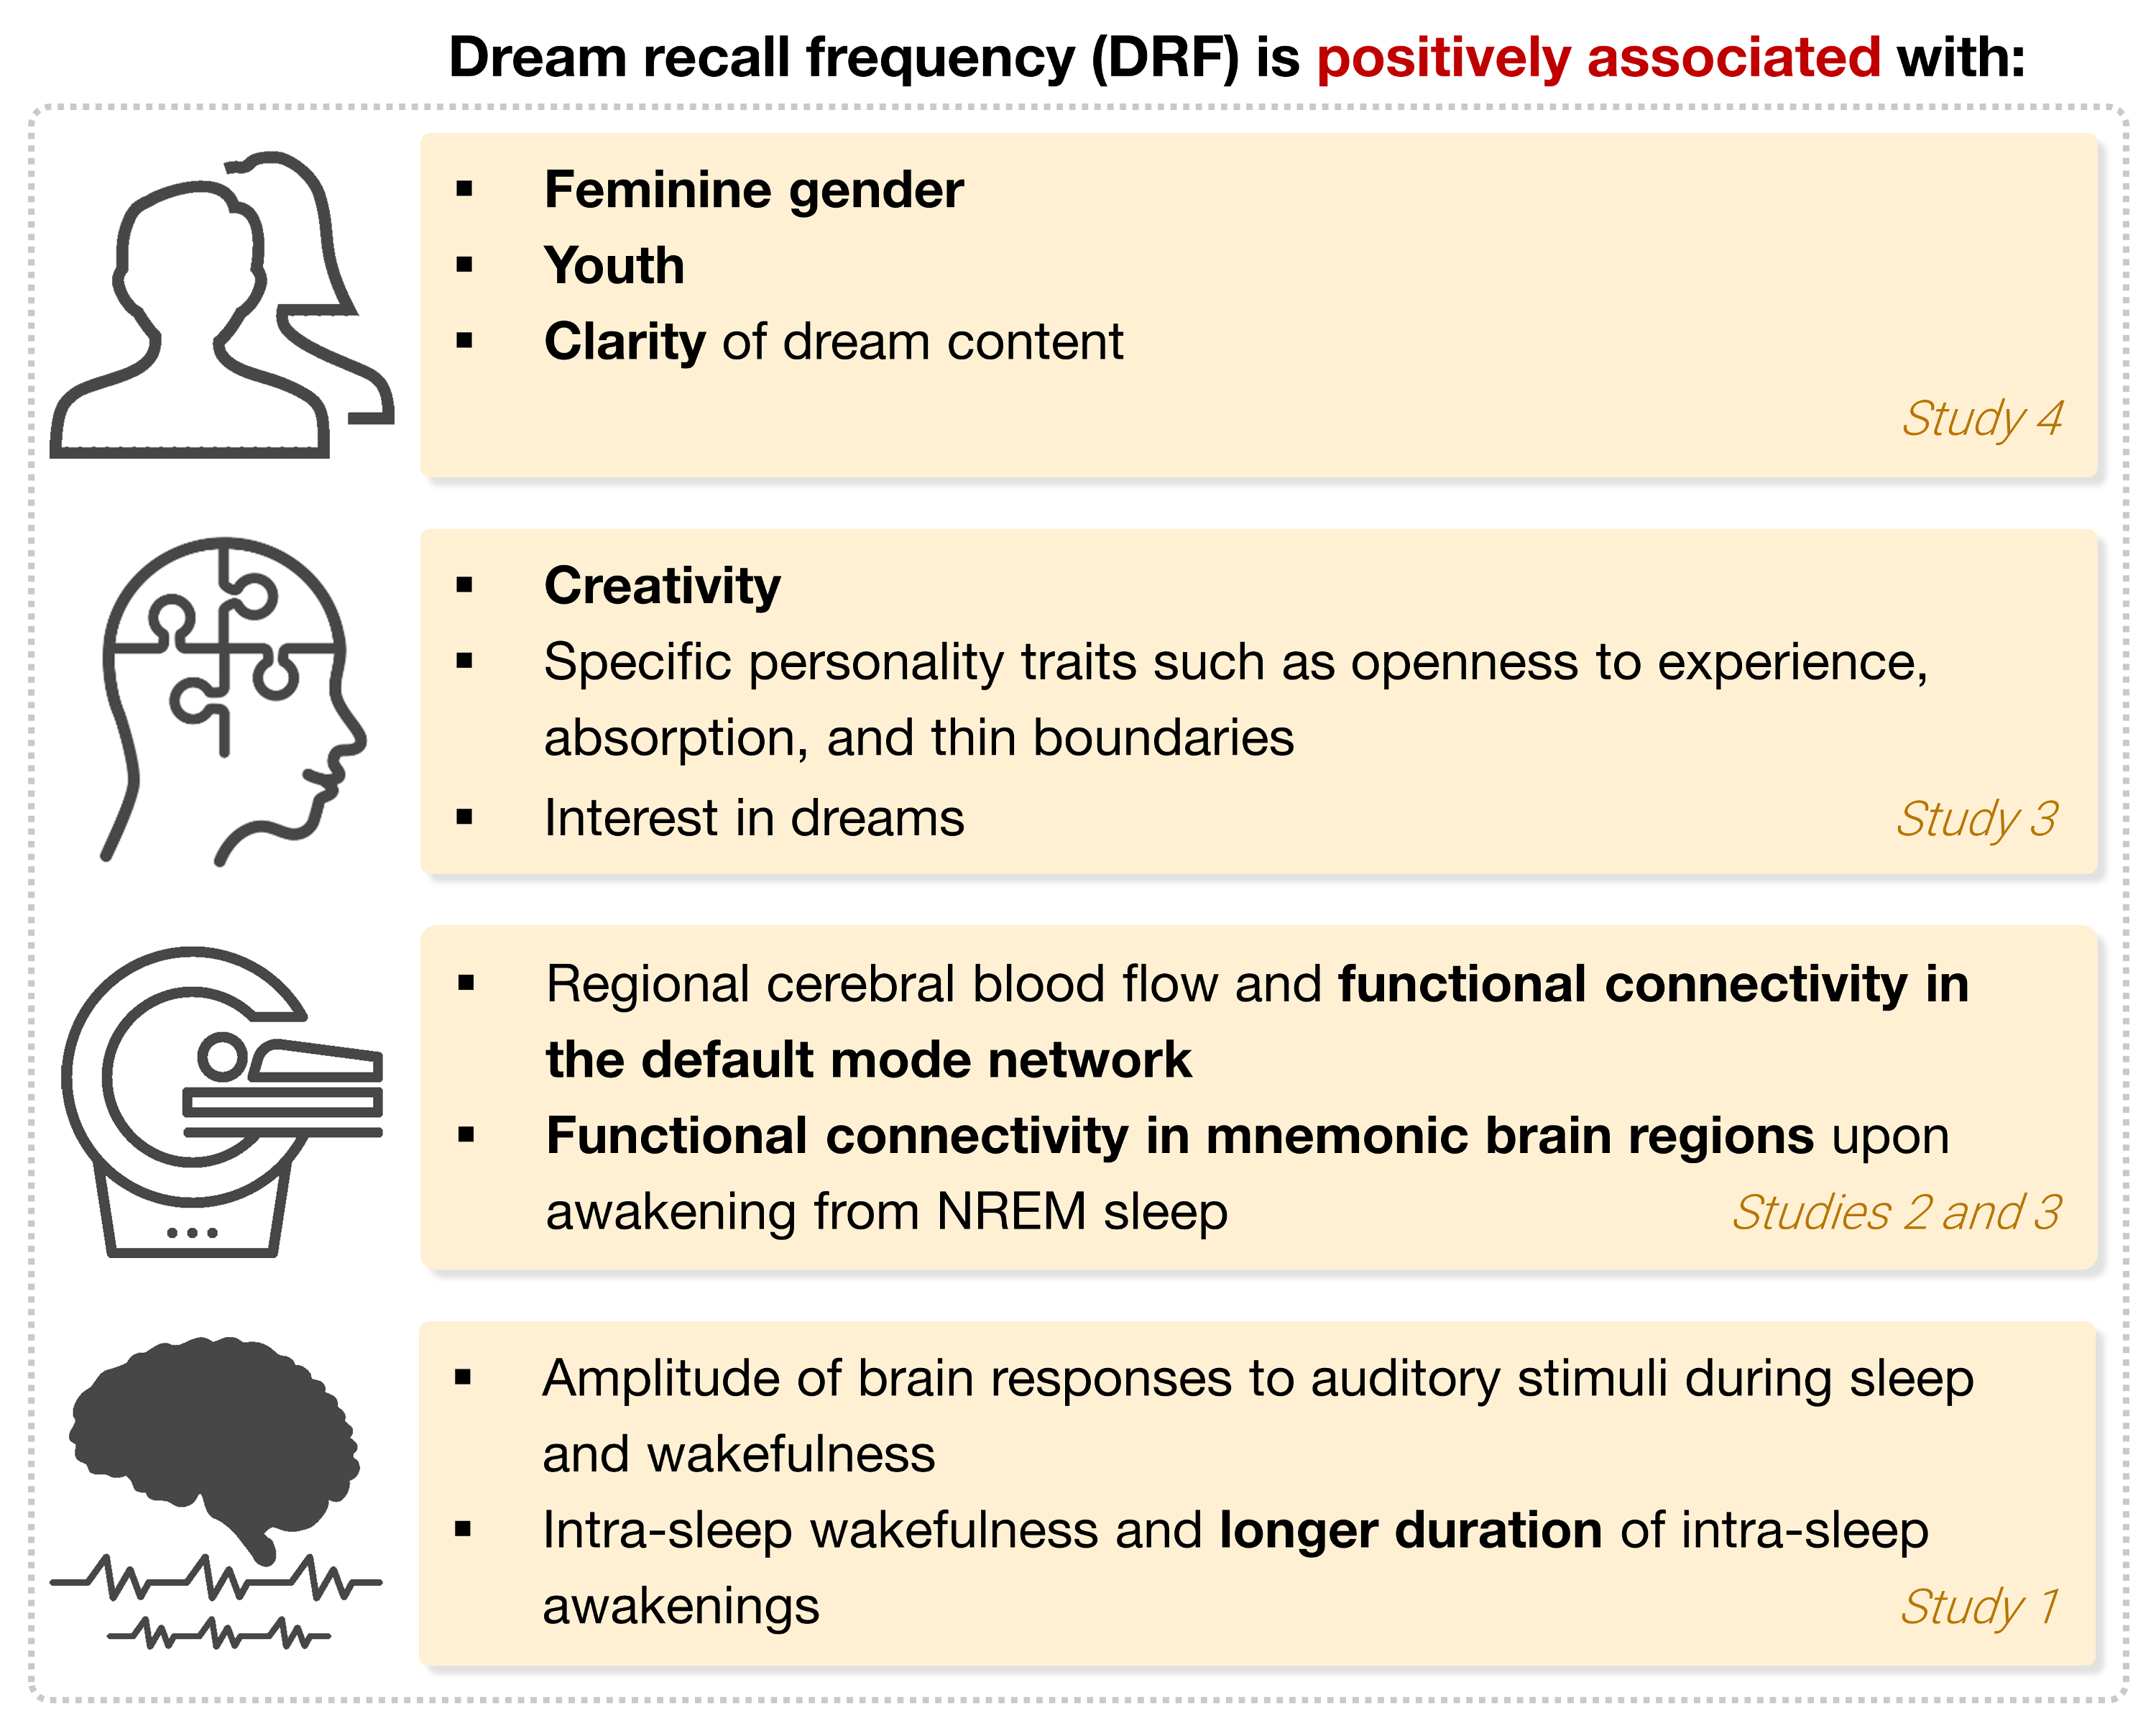
\includegraphics[width=\textwidth]{Fig/Discussion/HR_recap.png}
	\caption[Summary of the results on DRF]{\textbf{Summary of the differences observed between high and low dream recallers}. The findings of the present thesis are written in bold. By opposition, DRF was not associated with memory abilities or the density of certain sleep microstructural events such as rapid eye movements, muscle twitches, spindles and K-complexes.}
	\label{fig:disc:drf:summary}
\end{figure}

\subsection{DRF is positively associated with intra-sleep awakening}
\label{disc:drf:summary:arousals}

In Study 1, we performed an in-depth investigation of the sleep macro and micro-structure of HR and LR by re-analyzing the polysomnographic recordings of \citet{eichenlaub_brain_2014}. First, we did not find any significant between-group differences in any of the sleep microstructural features considered (e.g. arousals, spindles, K-complexes, REMs). Our interpretation of these findings is that, most probably, sleep microstructural features are not crucial factors to explain DRF variability.
By contrast, we observed that full awakenings (i.e > 15 seconds) were longer in all sleep stages in HR as compared to LR (roughly 2 vs 1 min respectively). Noteworthy, the number of awakenings was not different between the two groups.

These observations led us to propose that the duration of intra-sleep wakefulness seems to be one of the most critical predictor of inter-individual differences in DRF. This result provides a strong evidence in favor of the arousal-retrieval model (see section \ref{sec:dream-recall:theories:arousal}, \citealp{koulack_dream_1976}), which states that a short period of wakefulness has to occur immediately after dreaming in order to transfer the dream content from short to long term memory. Our findings constitute an essential contribution to this model by showing that awakenings must be of sufficient duration to allow successful encoding of dreams into memory. We proposed, in accordance with previous findings \citep{campbell_perception_1981}, that two minutes of wakefulness might be a threshold duration for the successful encoding of dreams into long-term memory.

On this point, it should be noted that the author of the present thesis contributed to an ongoing study aiming at investigating, by means of human intra-cortical EEG, the temporal dynamic of reactivation of brain regions involved in memory processing during arousals (ranging from 3 sec to 2 minutes). Preliminary results showed that the spectral composition of hippocampal EEG signal during these arousals was intermediate between that of sleep and wakefulness activities, and that this activation was modulated by the awakening duration. Furthermore, we observed that hippocampus activity during these arousals was different during NREM and REM sleep, a finding particularly relevant considering the well-known dichotomy between these two sleep stages with regards to dream recall and, more broadly, memorization processes \citep{nielsen_review_2000, conduit_poor_2004}.

The visual scoring of arousals allowed us to address another issue, which is related to the finding of differential brain reactivity to auditory stimuli in high and low dream recallers (see section \ref{sec:dream-recall:param:neuro}). \citet{eichenlaub_brain_2014} has suggested that there might be a causal link between the larger brain responses to auditory stimuli and greater intra-sleep wakefulness during sleep in HR as compared to LR. In other words, the amplitude of brain responses to auditory stimuli could be predictive of subsequent awakening or arousal reactions, an observation that has been previously reported for nociceptive stimuli \citet{bastuji_laser_2008}. To test this hypothesis, we computed the auditory evoked potentials to arousing stimuli (i.e. inducing either an arousal or awakening) or non-arousing stimuli (i.e. stimuli that do not induce a disruption of the PSG signal). This comparison was not possible without the tedious and time-consuming visual scoring of arousals, given that arousals are far more frequent than awakenings in a normal night of sleep and are therefore needed to compute reliable and statistically valid evoked potentials. Consistent with our hypothesis, we have shown that brain responses to auditory stimuli, in N2 sleep, were larger when followed by a subsequent arousing reaction. Importantly, this increase in the amplitude of the brain responses seemed to be stimulus-specific given that the amplitude was larger when arousing reactions were within 5 seconds after the stimulus compared to when they were between 5 and 15 seconds. Although it was not possible to compare the brain responses to arousing stimuli between HR and LR (because too few subjects in each group had a sufficient number of arousing stimuli), behavioral results show that HR elicited a significantly greater proportion of stimuli followed by an arousing reaction than LR.

In sum, our findings argue for the existence of a causal link between intra-sleep awakening and the brain reactivity to stimuli during sleep. As compared to LR, a greater brain reactivity during sleep in HR could promote intra-sleep awakening which could in turn promote dream recall. Our hypothesis is that if these awakenings are of sufficient duration to allow for the reactivation of the memory encoding abilities of the hippocampus, then the dream content will be successfully encoded into long-term memory and therefore lead to a successful dream recall. This hypothesis led us to address the broad issue of how the brain awakens from sleep, and specifically whether there are differences in this awakening process between HR and LR, an issue that we will discuss in the following section.

\subsection{DRF is positively associated with brain functional connectivity upon awakening}
\label{disc:drf:summary:inertia}

In Study 2, we tested the hypothesis of a differential sleep inertia between HR and LR. To this aim, we designed an EEG-fMRI sleep study to compare specifically the brain functional connectivity and cognitive performances of these two groups following awakening from a daytime nap. To our knowledge, this was the first study to experimentally test the relationship between sleep inertia and DRF.

While we were not able to evidence behavioral between-group differences in sleep inertia (discussed in section \ref{res:inertia:drf:discussion}), our results shed light on a differential brain functional organization associated with DRF in the minutes following awakening from sleep. We found that at 5 min-post-awakening, HR exhibited a greater functional connectivity within the default mode network and regions involved in memory retrieval, such as the medial prefrontal cortex (MPFC), the precuneus, the left medial temporal lobe (MTL) and the left dorsolateral prefrontal cortex (DLPFC). Remarkably, these are almost exactly the same regions found to be involved in episodic memory encoding and retrieval (reviewed in \citealp{spaniol_event-related_2009}). Our interpretation of these results is that the higher functional connectivity in mnemonic brain regions observed in HR could facilitate in these participants the retrieval of dream content. Inversely, LR could fail to recall their dreams because of greater functional connectivity alterations during the first minutes following awakening. More broadly, our results argue in favor of a differential functional awakening process between HR and LR that could explain inter-group differences in dream recall.

\subsection{DRF is positively associated with creative-thinking abilities and default mode network connectivity}
\label{disc:drf:summary:dmn}

There is a rising consensus that dreaming, or at least dream recall, could be underlain by regions of the default mode network (DMN). In Study 3, we re-analyzed the fMRI data of Study 2 to specifically investigate the relationship between DRF and the DMN. Our results show that, during rest and compared to LR, HR exhibit a higher functional connectivity within the DMN (1) in average and (2) specifically between the MPFC and TPJ. These results are remarkably consistent with previous ones showing a higher rCBF in HR between these two same regions during sleep and wakefulness \citep{eichenlaub_resting_2014}, and a cessation of dream reporting following focal lesions in these brain areas \citep{solms_neuropsychology_1997}. Based on all these observations, one can reasonably argue that the TPJ and the MPFC are two critical regions when it comes to the ability to recall dreams. The question remains pending whether these regions are only involved in dream recall during wakefulness, or also in the production of dreams during sleep. It would be premature to answer that question given that we still have no other means than awakening the participants to test whether he or she was dreaming before.

The second goal of this study was to compare the cognitive abilities (e.g. memory, creativity) and personality traits of HR and LR. We found that HR scored higher than LR on measures of creative-idea generation, without any further between group differences in memory or cognitive abilities. Regarding personality traits, we found that HR tended to score higher on several big five dimensions such as neuroticism, agreeableness and openness-to-experience. These differences were however not significant. This could be due, in part, to the number of participants (n=55), which despite being considerable for a typical neuroimaging study (especially involving simultaneous EEG-fMRI recordings), is rather low for behaviorally assessing subtle differences in personality traits (e.g. n=981 in \citealp{hartmann_boundaries_1989}). The finding of a higher creativity in HR than in LR, which has already been reported in several studies \citep{fitch_variations_1989, schredl_creativity_1995, schredl_factors_2003}, is particularly interesting given that creative-thinking has also been associated with a preferential recruitment of the DMN \citep{ellamil_evaluative_2012, jung_structure_2013, beaty_creativity_2014, mok_interplay_2014, beaty_default_2015, christoff_mind-wandering_2016}. As such, these findings are consistent with the emerging view that creative-thinking and dreaming share some phenomenological and neurophysiological properties \citep{christoff_mind-wandering_2016}.

Altogether, these results argue in favor of Schonbar's claim \citeyearpar{schonbar_differential_1965} that high or low DRF can be explained by the \q{life-style} of individuals (among which are creative-thinking abilities and personality traits). Our findings go one step further by suggesting that this life-style is related to a specific brain functioning, characterized notably by an increased functional connectivity in the DMN. As we will discuss in section \ref{disc:drf:model}, the question remains to whether there is a causal link between all these variables, and notably whether personality traits and life-style can significantly influence and modify the brain functional properties.

\subsection{DRF and age, sex, and clarity of dream content}
\label{disc:drf:summary:survey}

We took advantage of the recruitment questionnaire of the EEG-fMRI study on sleep inertia to perform an epidemiological survey of the sleep and dream habits of a large sample of French college students from Lyon University. The survey included several questions regarding DRF. Remarkably, we were able to evidence a negative correlation between DRF and age, even on the tight age range of our sample (i.e. from 18 to 30 years old), as well as a positive correlation between DRF and the clarity of dreams. Furthermore, we were able to replicate the finding of a higher DRF in women than in men \citep{schredl_gender_2008}. Many factors could explain, at least partly, this gender difference in DRF. For instance, \citet{schredl_gender_2008} proposed that it was the result of a gender-specific dream socialization process during childhood. According to them, girls are encouraged more often than boys to talk about their dreams during their childhood, and might therefore develop a stronger interest in dreams, a factor consistently reported to be positively associated with DRF \citep{schredl_factors_2003}. Another possible explanation could be the higher proportion of intra-sleep wakefulness reported in women as compared to men \citep{reyner_gender-and_1995}, which could give them more opportunities to encode dreams into memory according to the arousal retrieval-model \citep{koulack_dream_1976}. Finally, drawing from Schonbar's life-style hypothesis \citeyearpar{schonbar_differential_1965}, one can argue that the higher DRF in women could be the result of differential personality and cognitive traits between men and women. This observation is supported by studies showing higher levels of neuroticism, extraversion, agreeableness, and conscientiousness in women compared to men, as well as a tendency for higher creativity (reviewed in \citealp{schmitt_why_2009, baer_gender_2008}).

Remarkably, age, gender and clarity can all be related to a specific default mode network (DMN) functioning. For instance, women tend to exhibit a higher functional connectivity in the DMN \citep{bluhm_default_2008}. Similarly, in comparison with younger subjects, older people were consistently found to exhibit a global lower functional connectivity within the DMN \citep{damoiseaux_reduced_2008, koch_effects_2010}, a finding well in line with the observation of reduced mind-wandering abilities in older people \citep{jackson_mind-wandering_2012}. Finally, there is a rising consensus that DMN may be involved in visual imagery process \citep{andrews-hanna_functional-anatomic_2010}, thus suggesting that a high DMN activity could be causally linked to an increased clarity of the dream content. By extension, this coudl mean that DMN activity is directly related to the salience of dream content. We will discuss further these interactions between DMN functioning and other factors related to DRF in the next section, in which we propose an integrative model of dream recall based on ann these findings.

\section{An integrative model of dream recall}
\label{disc:drf:model}

How can we combine the above findings on DRF variability to the previously existing knowledge on dream recall?
The results of the present thesis led us to propose a comprehensive and integrative model of dream recall, depicted in Fig \ref{fig:disc:drf:model}.

The main assumption of this model is that successful dream recall requires the encoding, during the sleep-wake transition, of the dream short-term memory into a more stable long-term memory. As proposed by \citet{koulack_dream_1976} and since then confirmed in numerous studies, this process is not possible during sleep but only during wakefulness. Consistent with this, we reported earlier that DRF is positively associated with intra-sleep wakefulness, and notably with the duration of awakenings. This observation led us to propose that intra-sleep awakenings must be of sufficient duration to allow the reactivation of the memory encoding abilities of the brain. Apart from the duration, other factors come into play to either facilitate or prevent the encoding of dreams during the period following awakening from sleep.

First, state-factors such as sleep inertia, and the magnitude of the functional difference between the pre- and post-awakening brain state \citep{koukkou_dreaming:_1983} are negatively associated with successful encoding of dream content. Both these factors are related to the physiological context, which include notably the prior sleep stage and sleep duration, the level of sleep deprivation and the time of the night (i.e. circadian factor). Second, as proposed by \citet{cohen_dream_1973}, the dream memory trace remains so long as there is no distraction or interferences in the encoding process. According to our model, the level of interferences could be directly related to traits factors, such as the interest in dreams. For instance, individuals highly interested in their dreams will probably make a voluntarily effort to \emph{grasp} the dream memory, and at the same time avoid interferences in the encoding process. This relationship could explain why DRF is known to be significantly enhanced by keeping a dream diary \citep{schredl_questionnaires_2002}.

Another factor that, according to our model, plays a crucial role is the salience of the dream content. This idea first proposed by \citet{cohen_test_1974} and received further support from experimental studies since then \citep{cipolli_bizarreness_1993, schredl_emotions_1998}. Put it simply, this hypothesis states that the more salient a dream is (e.g. vivid, bizarre, emotionally intense), the more likely it will be recalled. This is well in line with the previously mentioned correlation between DRF and clarity of dream content. Furthermore, our model incorporates Schonbar's life-style hypothesis \citeyearpar{schonbar_differential_1965} to postulate that all these processes (e.g. salience, interference, sleep inertia) are influenced by the life-style, personality traits and cognitive abilities (e.g. creativity) of the dreamer.

One of the key finding of the present thesis is that these differential cognitive and personality profiles between high and low dream recallers are also associated with a specific brain functional organization, characterized notably by a higher DMN activity in high dream recallers. According to our model, this specific neurophysiological profile could promote in HR some cognitive abilities such as creativity, which would in turn increase the salience of dream content and promote intra-sleep awakenings. These two factors, associated in HR with reduced brain functional alterations and interferences upon awakening, could facilitate the encoding of dreams and result in an increased dream recall frequency. Lastly, some studies indicate that (1) women score higher on certain personality traits and exhibit a higher DMN functional connectivity (2) aging is negatively associated with cognitive functioning and DMN activity. For these reasons, we believe that age and sex influence, at the lower level, all the following factors related to the process of dream recall.

\begin{figure}[!htbp]
	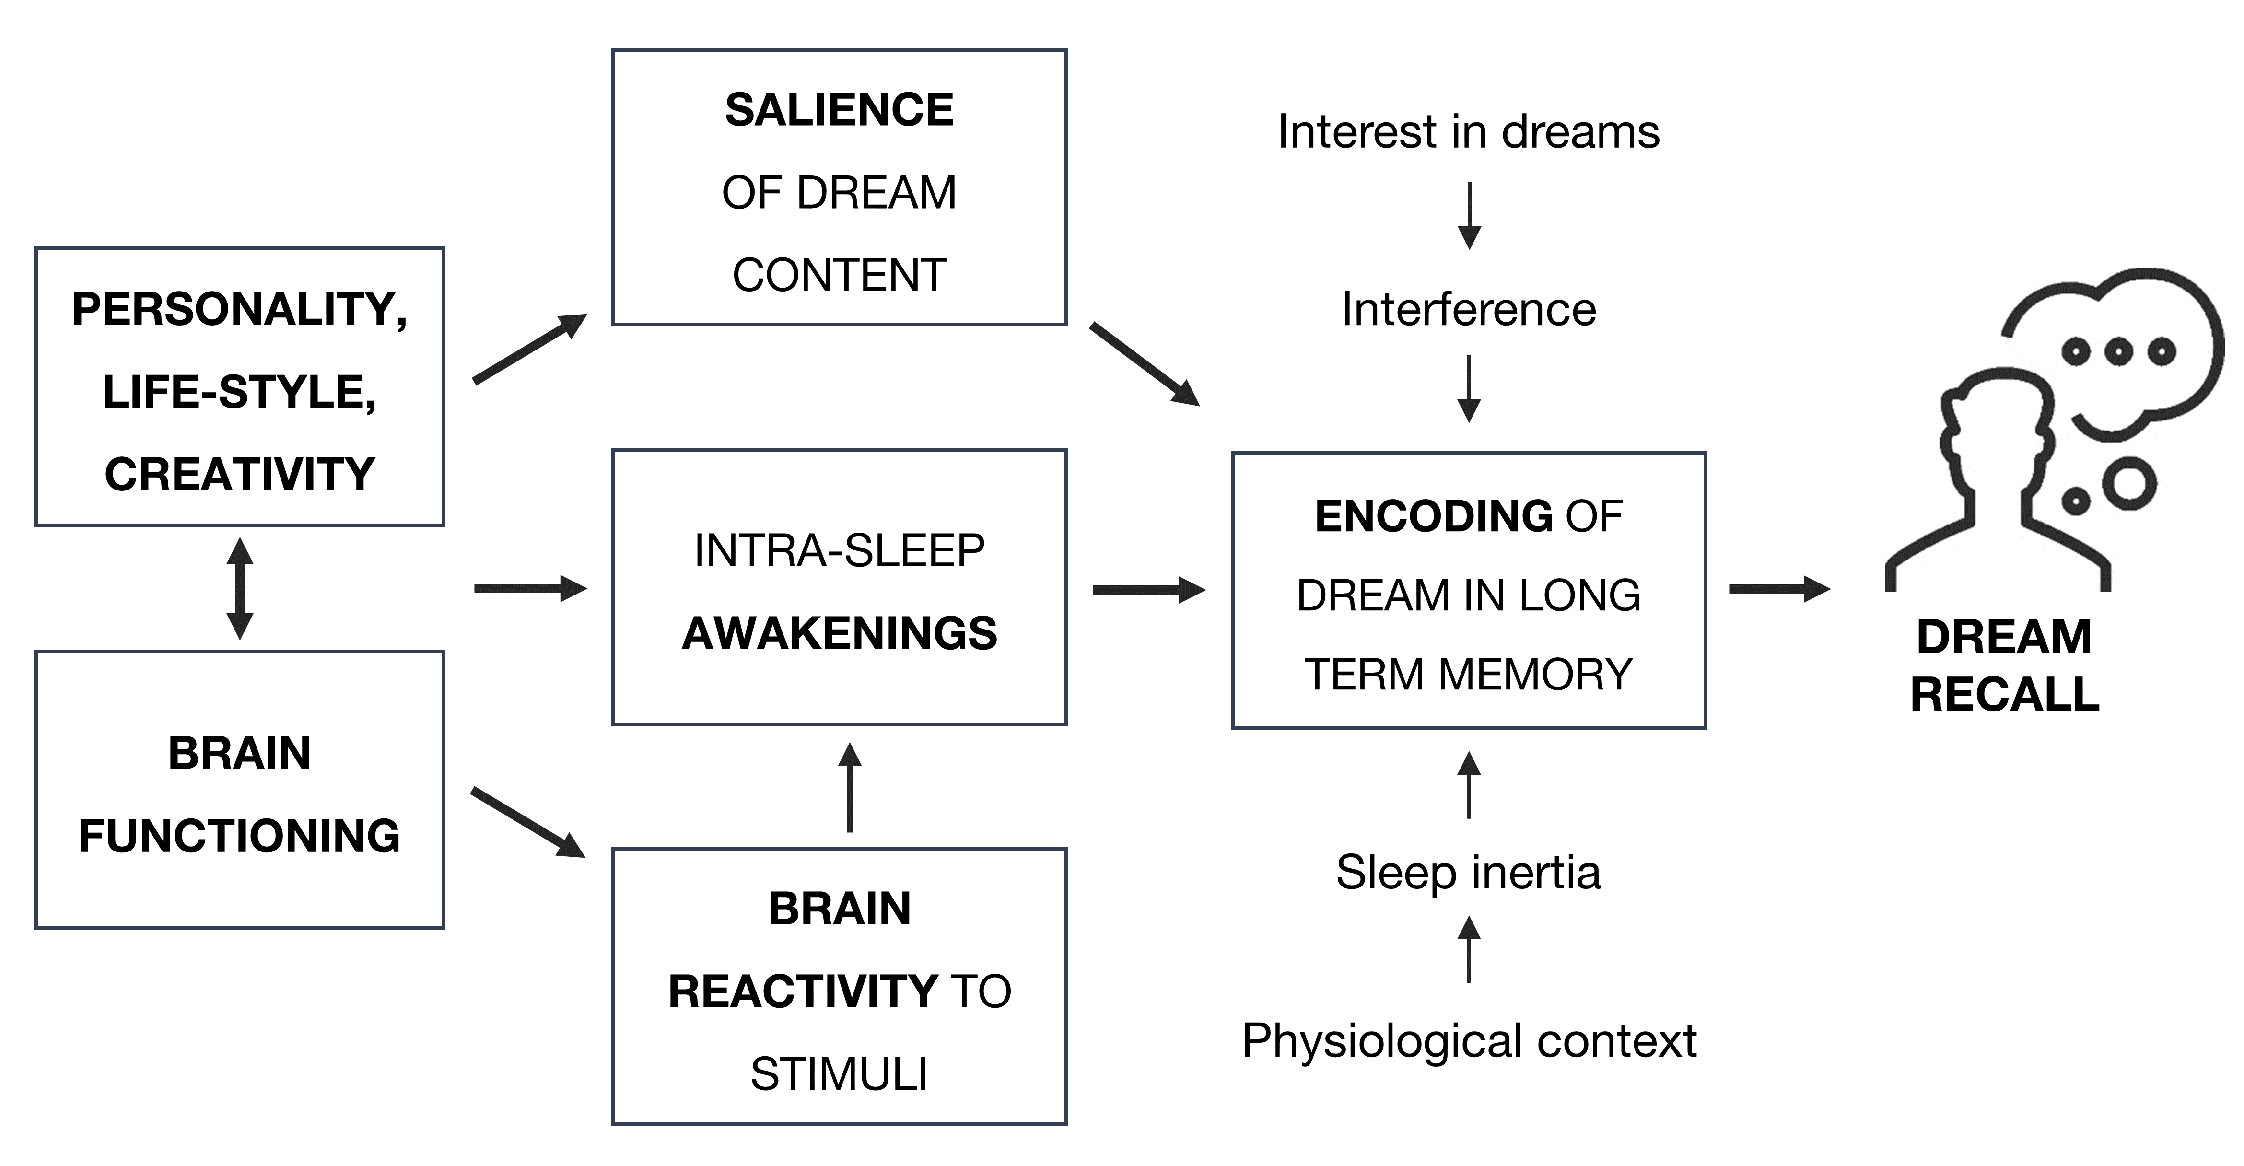
\includegraphics[width=\textwidth]{Fig/Discussion/schema_dream_recall.png}
	\caption[An integrative model of dream recall]{An integrative model of dream recall.}
	\label{fig:disc:drf:model}
\end{figure}

\section{Conclusions and perspectives}
\label{disc:drf:perspectives}

In summary, the different studies of the present thesis significantly improved our knowledge of the factors and their interactions contributing to the process of dream recall. Based on the latests experimental findings, we proposed an integrative model of dream recall which can serve as a basis for future work. Among possible future axes of research, it seems promising to test whether DMN activity could also predict intra-individual variability in DRF across time. To this aim, one could use DRF enhancing methods (such as keeping a dream diary; \citealp{schredl_questionnaires_2002}) to test whether an increased DRF would result in increased creativity scores and DMN functional connectivity in post compared to pre-training measures within the same individuals (preferentially an initial group of low dream recallers).

%%%%%%%%%%%%%%%%%%%%%%%%%%%%%%%%%%%%%%%%%%%%%%%%%%%%%%%%%%%%%%%%%%%%%%%%%%%%%%%
\cleardoublepage
\chapter{The relationship between waking life and dream content}
\label{disc:wle}

\section{Such stuff as dreams are made on}
\label{disc:drf:summary:residue}

\myepigraph{We are such stuff,\\ As dreams are made on; and our little life, \\ Is rounded with a sleep}{William Shakespeare}{The Tempest. 1611}

Through an extensive investigation of the relationship between waking-life and dream content, Study 5 significantly improved our knowledge of the \emph{stuff that dreams are made on}. We asked participants to record and describe, over a period of one week, the obvious connections that they could make between their waking-life and dream content. By specifically investigating the characteristics of waking-life experiences (WLE) incorporated into dreams, we enhanced our understanding of the filter that dreaming applies to waking life.

We observed that the \q{dream mixture}, as Freud called it, is composed of various and opposite WLE which are all incorporated in significant proportions, i.e. recent and old, emotionally loaded and emotionless, positive and negative, important and insignificant, concerns and non-concern issues, to name but a few. Remarkably, we also found a significant interaction between the temporal remoteness of WLE and their emotional intensity. Older memories were scored by the subjects as the most emotionally intense and important, by opposition with memories of the day before (i.e. day-residues) that were mainly self-rated as non-important and emotionally neutral. These observations led us to support \citet{payne_sleep_2004}'s claim that dream content reflects certain memory processes taking place during sleep. Notably, the selective consolidation and/or forgetting of new memories during sleep (i.e. \q{memory triage}, \citealp{stickgold_sleep-dependent_2013}) could be function of the adaptive relevance and the emotional intensity of these memories \citep{schwartz_are_2003, malinowski_memory_2014, saletin_role_2011}.

\section{A role of dreaming in emotional regulation}
\label{disc:drf:summary:regulation}

The questionnaires that the participants had to fill in each morning after awakening included questions regarding the emotional tone of the waking-life memories, not only as they were experienced originally, but also as they were experienced within the dream content. Remarkably, we found that the dreamed version of the WLE was emotionally down-regulated compared to its waking-life counterpart form. Both emotionally positive and negative WLE were rated as more neutral within dreams as compared to their original occurrence in waking-life.

These results suggest the existence of a down-regulation of emotional waking memories during dreaming (i.e. attenuation of the emotional intensity of waking memories toward a more neutral tone), and provide as such one of the very few experimental evidences supporting the emotional regulation theory of dreaming \citep{cartwright_role_1998, cartwright_role_1998-1, perogamvros_roles_2012}, which claims that dreaming may actively moderate mood overnight in healthy individuals (see section \ref{sec:dream-func:modern:emotion}). While the emotional regulation function of sleep is well-known \citep{goldstein_role_2014}, results from our study further suggest that dreaming \emph{per se} may be involved in emotional regulation process, notably through the down-regulation of the affective tone of emotional waking memories.

On this point, it is noteworthy that a recent ERP study suggested a dissociation between the informational and emotional components of memories during REM sleep, which might, according to the author, result in a strengthening of the informational core of the memories combined with a reduction of the affective tone \citep{groch_role_2013}. From this finding, one can either argue that dreaming  reflects this mechanism (yet only found during REM sleep), or that dreaming is actively involved in this mechanism. If so, the down-regulation of emotional memories during dreaming could be accomplished via a similar dissociation between the original emotional and perceptual content of the WLE, a prediction consistent with the results of our study. We will conclude this section by mentioning the intriguing idea that in addition with being involved in mood regulation, this recombination of memories may also lead to creative insights and new ideas \citep{maquet_psychology:_2004, payne_sleep_2004, edwards_dreaming_2013, barrett_dreams_2017}. All the more reason, then, to believe that Hamlet is right to say \q{to sleep, perchance to dream} (Shakespeare, Hamlet, 1603).

\section{Perspectives}
\label{disc:drf:summary:perspectives}

Several open questions remain following this work. For instance, several studies demonstrated that time of night affects wake–dream continuity \citep{roffwarg_effects_1978, malinowski_effect_2014}, with notably a preferential incorporation of memories from the recent past in the beginning of the night, and a preferential incorporation of memories from the distant past in the end of the night. This suggests the thought-provoking idea that consolidation and regulation processes of waking memories follows a sequential pattern throughout the night. Accordingly, novel and salient waking memories from the recent past could be prioritized and processes earlier in the night than old memories. It would be thus interesting to test, using our protocol, whether we could find differences between the characteristics of the WLE observed from spontaneous awakening (i.e. at the end of the night) and those of the WLE observed earlier in the night (for example, by asking participants to put an alarm clock 2 or 3 hours after going to bed).

Another, perhaps more theoretical issue, relates to whether the dream does really incorporate both day-residues and old memories, or rather that these old memories are somehow linked to day-residues. This latter idea was proposed by \citet{freud_interpretation_1900} who noticed that \q{references to earlier episodes in life may also be incorporated [into dreams], but these episodes were always linked somehow to the dream-day and were therefore, day-residues. For example, they could have been recalled during the dream-day or perhaps reflect the same concern as the day-residue} \citep{marquardt_empirical_1996}. This problem has also been raised by \citet{grenier_temporal_2005} who proposed that \q{it would be interesting to examine the profile of references [i.e. WLE] that were identified as having been recently thought of or talked about, and to trace the life period to which they refer in terms of the last time seen or experienced in reality}. The issue remains, however, as to whether the participants would be able to remember all their daily thoughts, words and deeds.

%%%%%%%%%%%%%%%%%%%%%%%%%%%%%%%%%%%%%%%%%%%%%%%%%%%%%%%%%%%%%%%%%%%%%%%%%%%%%%%
\cleardoublepage
\chapter{Methodological development}
\label{disc:methods}

\section{A state-of-the-art open-source software}
\label{disc:methods:software}

SLEEP is a free, cross-platform and open-source graphical user interface dedicated to sleep reading, scoring and analysis. Initially designed for a personal use, it soon extended into a fully developed module with a comprehensive and intuitive interface. SLEEP has many advantages over other existing solutions. First, and perhaps most importantly, it is free and open-source. Second, it leverages the graphics processing unit to deliver cutting edge graphical performances. Third, it natively supports several commercial and public data file formats, thus making it accessible to the greatest possible number of people. Fourth, it implements several signal processing tools, as well as several automatic detections of sleep microstructural features. Fifth, it comes with an extensive documentation, a chat room and a peer-reviewed publication. In view of all these functionalities, one can reasonably conclude that SLEEP represents a state-of-the-art software in sleep research which should consequently benefit many. Furthermore, as the development of the software is still ongoing, novel functionalities will continue to be added. Some of these future perspectives are detailed in the section below.

\section{Future directions}
\label{disc:methods:future}

SLEEP includes so far 5 algorithms for detecting some of the most prominent features of each sleep stage, namely spindles, K-complexes, slow waves, rapid eye movements and muscle twitches. Two of these detections (spindles and K-complexes) were compared against a visual scoring reference and showed overall good performances. Yet, there are still opportunities for further enhancements and the detection algorithms were improved since the initial, published, version. An example of the updated spindles detection pipeline can be found in Fig \ref{fig:disc:methods:future:spindles}.

\begin{figure}[htb]
	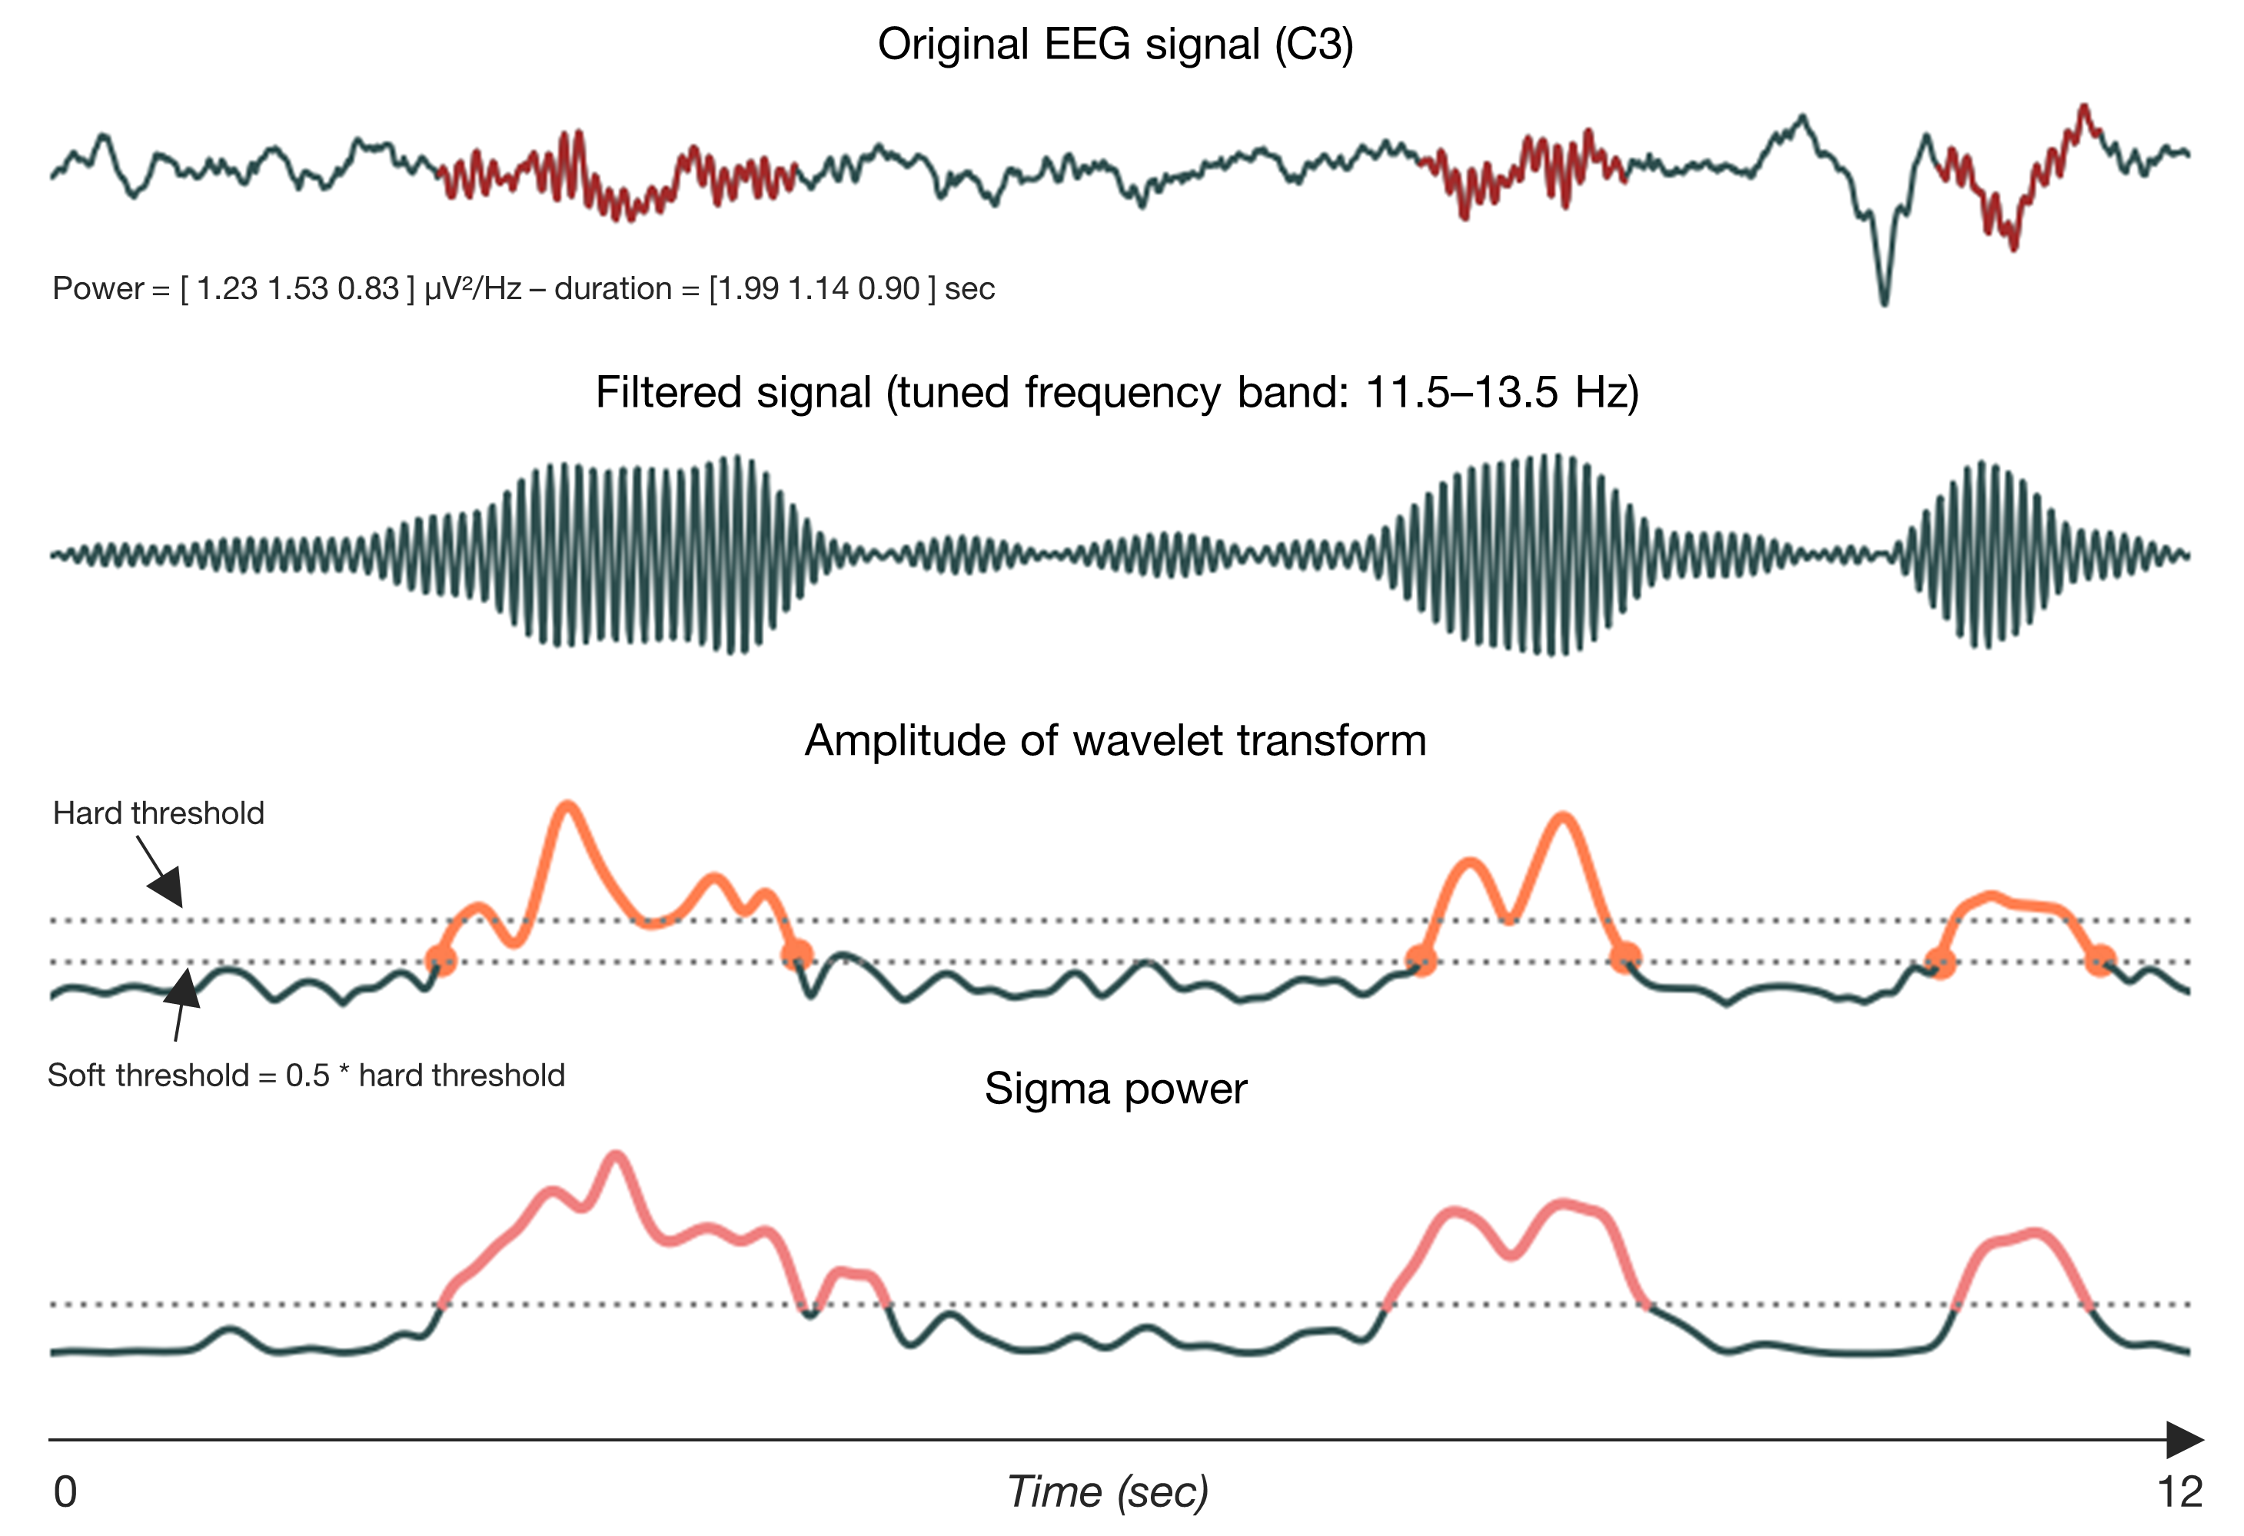
\includegraphics[width=\textwidth]{Fig/Discussion/spindles.png}
	\caption[Improved spindles detection algorithm]{\textbf{Improved spindles detection algorithm.} Compared to the initial algorithm (presented in chapter \ref{res:software}), the new spindles detection has several improvements. First, we implemented a data-driven tuning of the spindle frequency band by finding the peak spectral power within the sigma range. This step, described by \citet{berthomier_automatic_2007}, allows to accommodate for inter-individual variability of EEG signals, and is particularly useful when analyzing patients who tend to exhibit higher variability. Second, we now use both a hard and a soft threshold on the amplitude of the wavelet transform to determine more precisely the beginning and the end of each spindle. Finally, to allow users to better understand how the detection algorithm works, we implemented a function to plot the current figure for each desired time window.}
	\label{fig:disc:methods:future:spindles}
\end{figure}

Furthermore, perhaps one of the most challenging issue in sleep research is the scoring of sleep stages. Currently, the gold standard remains visual scoring by an expert, which is time-consuming and subject to high inter-rater variability. There is therefore a crucial need for reliable and time-efficient algorithms capable of detecting sleep stages in healthy and patients alike. With this in mind, we are currently working on two distinct automatic sleep scoring methods, based respectively on spectral feature extraction / microstructural detection (Fig \ref{fig:disc:methods:future:autoscore}), and on machine-learning algorithms. Preliminary results based on the former method show a 81\% agreement with a manually scored standard reference, a figure comprised within the range of human inter-scorer agreements (generally between 80 and 90\%, see \citealp{silber_visual_2007}). A similar agreement was obtained using the second, machine-learning based automatic sleep scoring method. Future developments will be needed to get the most out of these two methods and ultimately provide a state-of-the-art algorithm.

\begin{figure}[htb]
	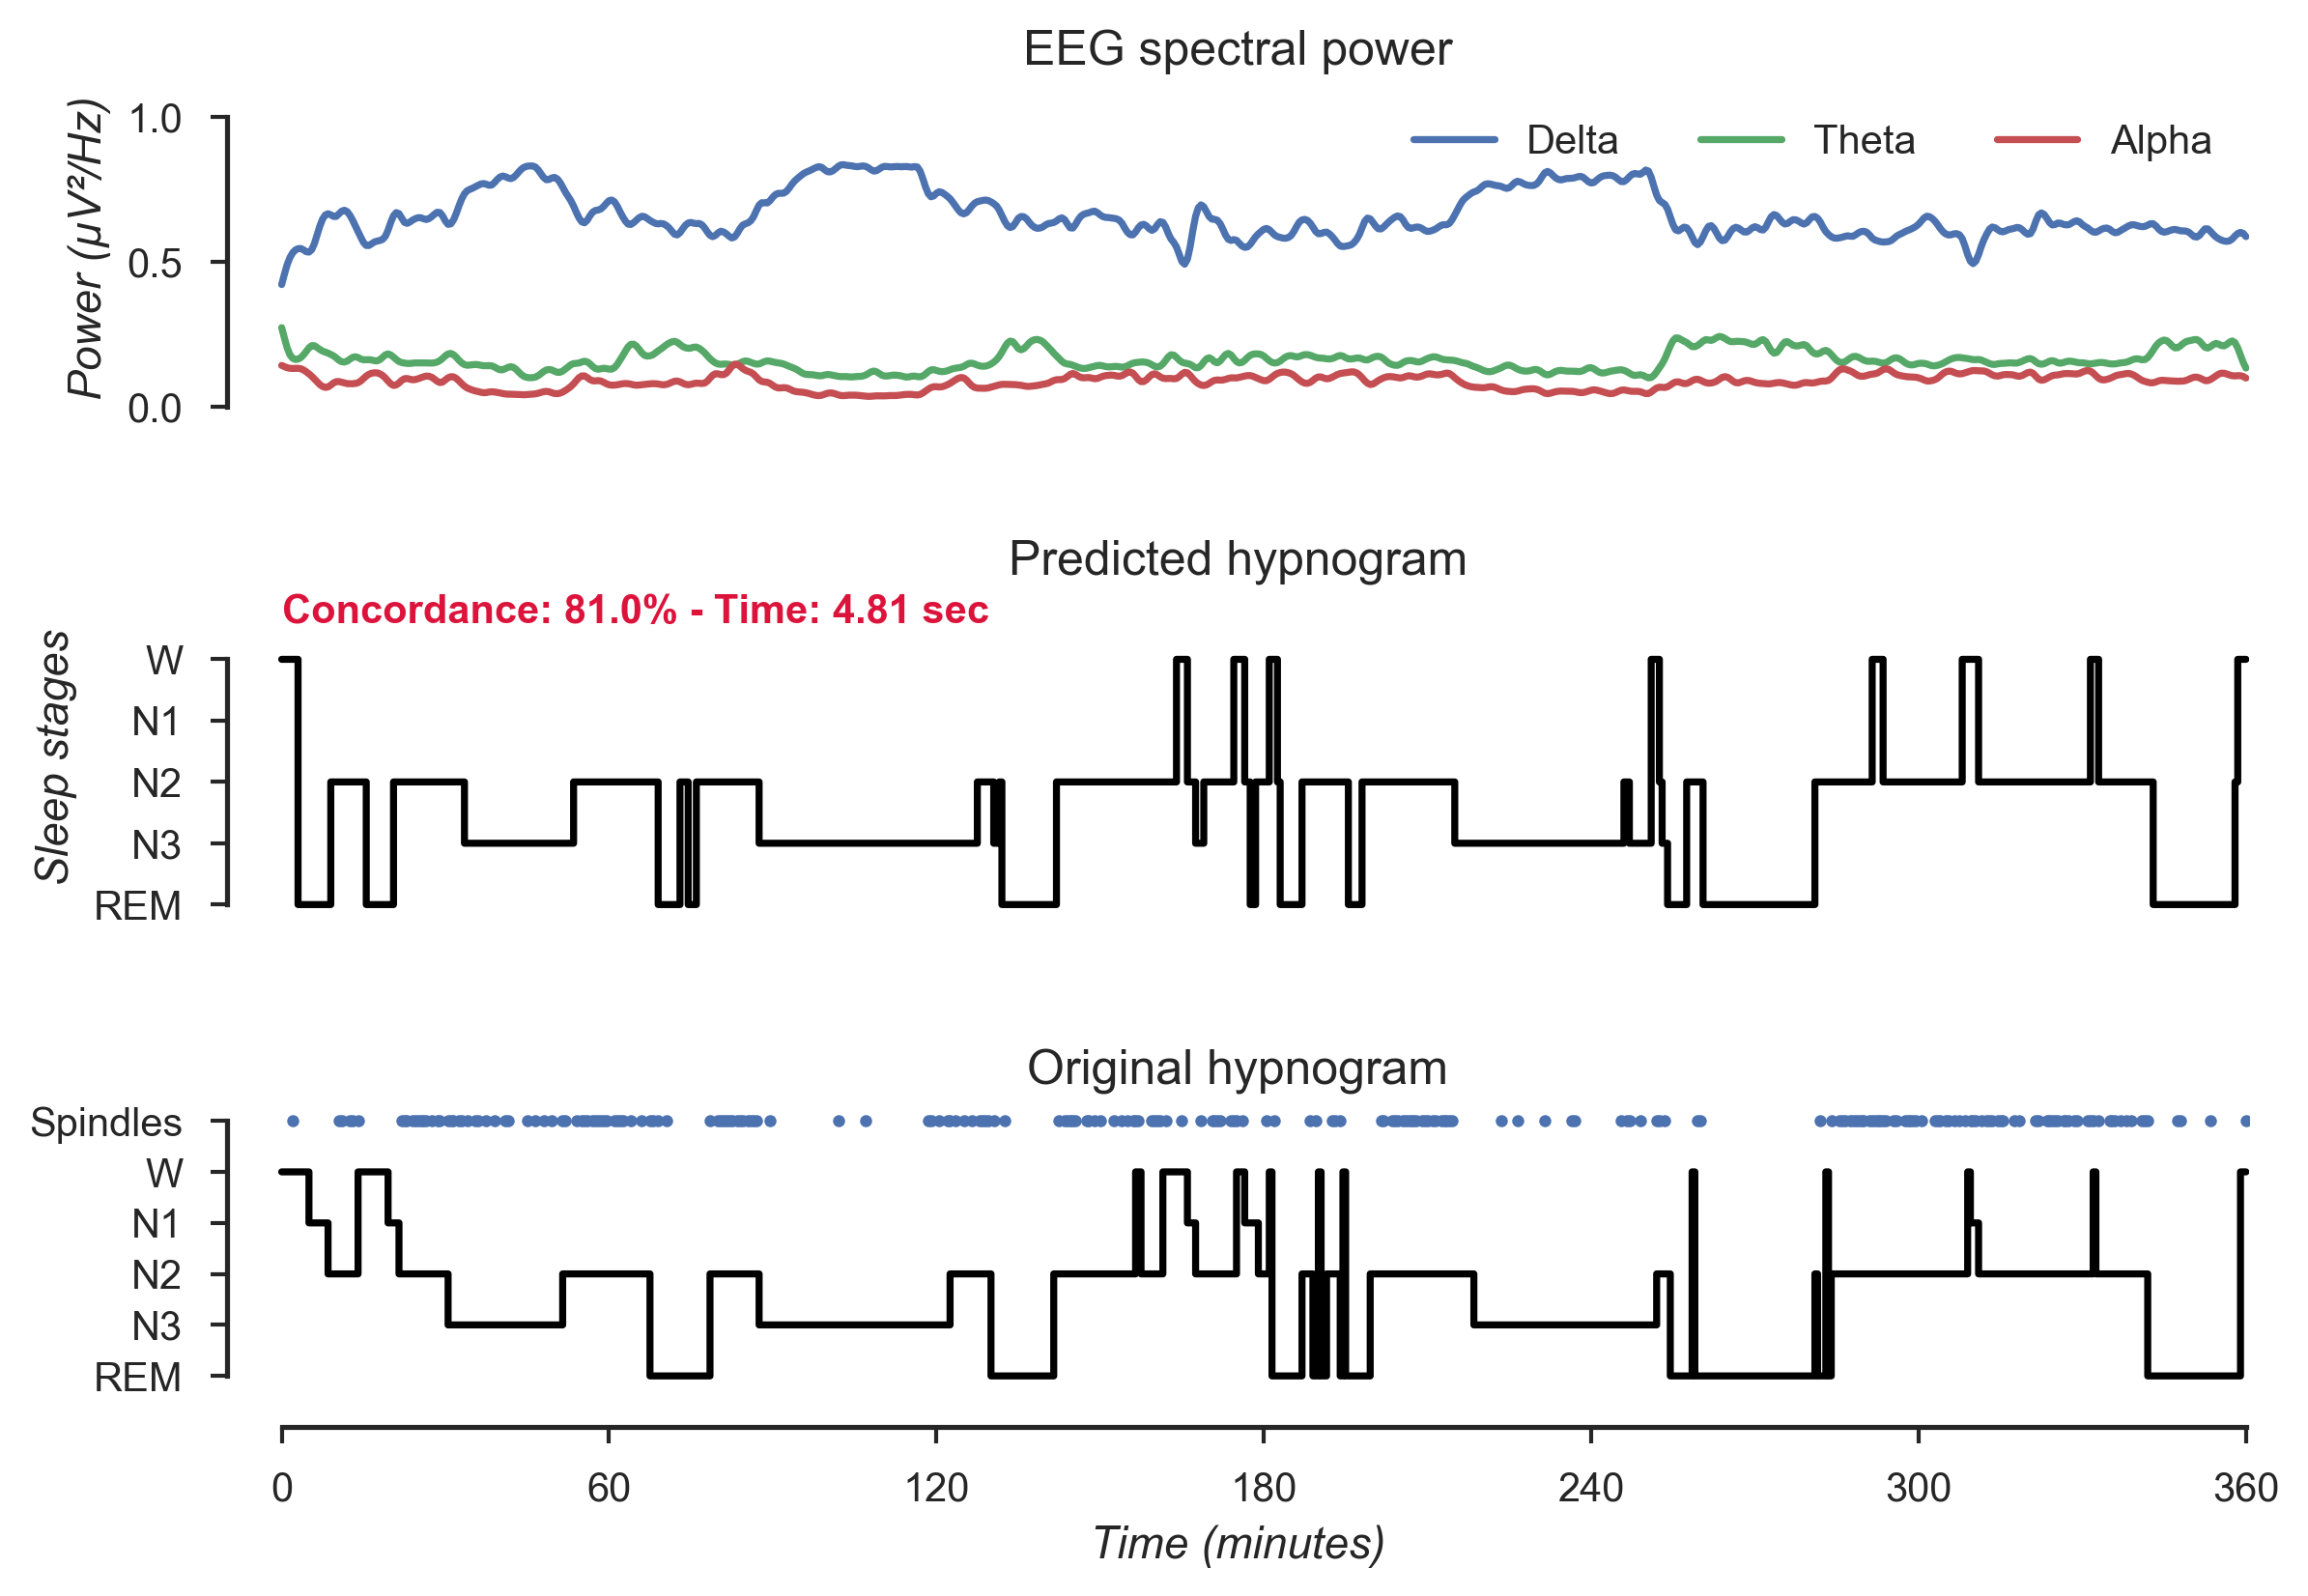
\includegraphics[width=\textwidth]{Fig/Discussion/autoscore.png}
	\caption[Preliminary results of the automatic sleep scoring algorithm]{\textbf{Preliminary results of the automatic sleep scoring algorithm.} The algorithm is based on a combination of spectral features extraction (Top) and automatic detection of microstructural features (e.g. spindles, blue dots). Preliminary tests on a single EEG channel (C3) of one healthy individual yielded 81\% agreement between the predicted and the manually scored full night hypnogram (with a running time inferior to 5 seconds).}
	\label{fig:disc:methods:future:autoscore}
\end{figure}

Because this software represents one of the very few open-source, free and exhaustive solution for sleep reading, scoring and analysis, it will probably reach in the near future a large public of sleep researchers, students and engineers, and hopefully lead to many great collaborations. These collaborations will be facilitated by the wide range of natively supported file formats, which allows sleep laboratories across the world to visualize and analyze their sleep data using a single, common software. In conclusion, we believe that the development of SLEEP represents a major step forward in sleep research, and more broadly in the emerging philosophy of open science.

%%%%%%%%%%%%%%%%%%%%%%%%%%%%%%%%%%%%%%%%%%%%%%%%%%%%%%%%%%%%%%%%%%%%%%%%%%%%%%%
\cleardoublepage
\chapter{General conclusion}
\label{disc:conclusion}

Throughout this work, we have addressed several unresolved issue related to the nature, the correlates and the function of dreaming. A large part of the present thesis was devoted to comparing cognitive and neurophysiological variables in high and low dream recallers, in an effort to understand \q{what cause sleepers sometimes dream, and sometimes do not} (Aristotle, On Sleep and Sleeplessness, 350 B.C., see section \ref{sec:dream-recall}). Our results revealed that the ability to recall dream is positively associated with (1) intra-sleep wakefulness during sleep, (2) the strength of functional connectivity in specific areas of the brain during sleep, wakefulness, and the sleep inertia period following awakening, (3) creative-thinking abilities. Based on all these findings, we proposed a new model of the dream recall process integrating the contribution of all these factors as well as their interactions.
